% this file is called up by thesis.tex
% content in this file will be fed into the main document

\chapter{Implementation} % top level followed by section, subsection

\section{OpenCSD}

In this section we describe the tools and techniques used with the OpenCSD
framework, detail modules with their respective functionality and show the
external dependencies as well as internal relationships of these modules. 
Followed by, sections on filesystem and offloading implementation details.

\subsection{Framework}

Firstly, OpenCSD consist of many external dependencies, most prominently
\textit{Storage Performance Development Kit} (SPDK) \cite{spdk},
FUSE \cite{fuse} and uBPF \cite{ubpf}. These technolgies are used as userspace
NVMe SSD driver and as virtual machine for the eBPF ISA respectively. Reusing as
many as pre-existing technologies as possible increases the change of
familiarity aiding ease of use. More prominently, these existing technologies
dramatically lower the amount of development effort required to create the
prototype. However, our design requirements demand these dependencies be
installed in an isolated way. To do this OpenCSD configures an isolated build
environment with dependencies made available through an environment file.
Moreover, this file configures variables such as \textit{PATH} and
\textit{LD\_LIBRARY\_PATH}. In addition, OpenCSD offers a QEMU installation and
accompanying qcow image to emulate a ZNS SSDs. This is to overcome the limited
availability of these SSDs as stated in the design requirements. However, the
use of QEMU for ZNS SSDs is entirely optional. Finally, CMake \cite{cmake} is
used to orchestrate the installation of dependencies as well as the compilation
of binary targets. Due to limitations it is advised to rerun CMake after each
make command, as this  prevents unnecessary recompilation of external
dependencies \footnotemark[11]. The combination of this isolated dependencies
environment managed through CMake with the ability to use QEMU for ZNS SSDs
emulation is ideal to minimize the complexity as exposed to users of OpenCSD.

\footnotetext[11]{Due to limitations in the evaluation of file presence
conditions which are not reevaluated when executing the generated makefile.}

As said OpenCSD is comprised of modules using a component architecture.
Additionally, Each module is compiled as a static or shared library to reduce
coupling. This creates an explicit nature of exchanging information between
linked libraries that allows to identify feasibility problems at an early stage.
This is opposed to potentially only identifying such issues when creating a
first hardware prototype. A trivial example of such infeasibilities would be
using shared memory mutexes to synchronize filesystem and CSx kernel behaviour.
Several modules are solely an interface with subsequent modules being one or
more concrete implemenations of these interfaces. These module based interfaces
with loose coupling allow for simplified replacement of technologies.

\subsubsection{Modules}

The overall modules of OpenCSD are shown in figure
\ref{figure:moduledependencies} along with any external or internal
dependencies. In addition, we briefly describe the functionality of each module.
Finally, at the end of this subsection we describe the three most prominent
modules of OpenCSD.

% Diagram with overview of different modules and their used as well as
% relationships. Also show integration of open-source technologies.

\begin{figure}
    \centering
	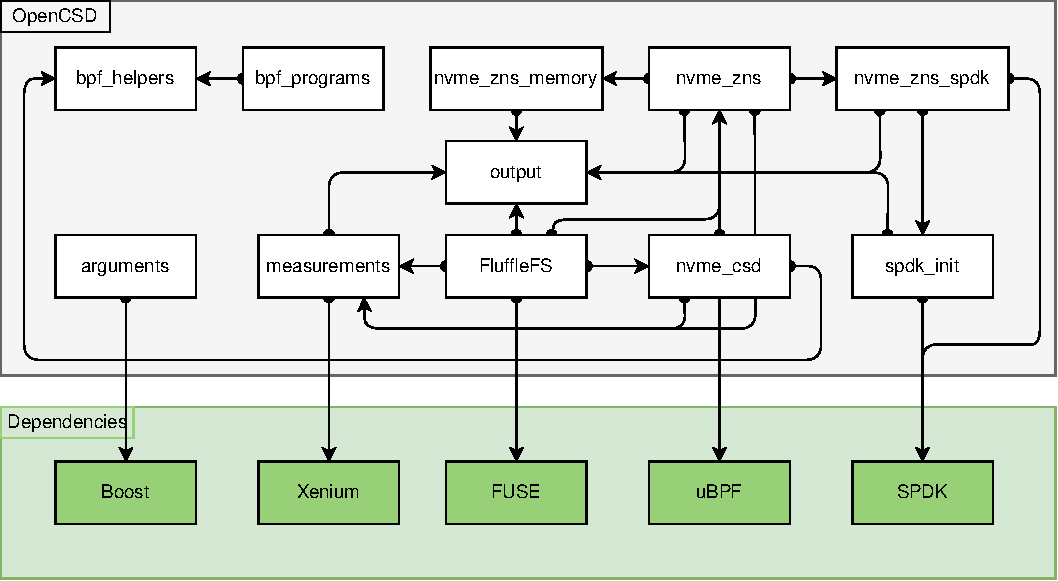
\includegraphics[width=1\textwidth]{resources/images/module-dependencies.pdf}
	\caption{Overview of all OpenCSD components and their depends-on relations}
    % \includesvg[width=0.6\columnwidth]{resources/images/module-dependencies}
    \label{figure:moduledependencies}
\end{figure}

\begin{itemize}
    \item output - Manages stdout and stderr output to the console by
    registering namespaces and providing a variety of log levels.
    \item arguments - Parses command line arguments and splits these into parts
    that can be passed to other modules in a decoupled nature. 
    \item measurements - Low overhead performance instrumentation for functions
    separated by namespaces using high performance lockless unbounded queue
    \cite{Michael1996SimpleFA}.
    \item spdk\_init - Collection of helpers to perform SPDK initialization and
    select ZNS suppporting NVMe namespace.
    \item nvme\_zns - NVMe interface to perform ZNS operations read, write and
    reset. To be used by FluffleFS for decoupled I/O operations.
    \item nvme\_zns\_memory - Memory backed implementation of nvme\_zns
    interface.
    \item nvme\_zns\_spdk - SPDK backed implementation of nvme\_zns interface
    \item nvme\_csd - Simulated extension to the PCIe NVMe protocol that allows
    to perform CSx operations. Execution of kernels is handled through uBPF.
    Utilizes instance of nvme\_zns to perform actual I/O operations performed by
    kernel.
    \item bpf\_helpers - Collection of headers that define the eBPF ABI
    supported for CSx kernels. ABI to be implemented by device vendor
    or in this case nvme\_csd for simulation. The ABI is filesystem agnostic.
    \item bpf\_programs - Collection of eBPF programs linked at runtime for
    previous ZCSD \cite{lukken2021zcsd} prototype.
    \item FluffleFs - FUSE LFS supporting in-memory snapshots to achieve
    multi-user tenancy with concurrent regular and offloaded filesystem access.
    Utilizes, nvme\_zns and nvme\_csd to achieve functionality.
\end{itemize}

Out of these components nvme\_csd, bpf\_helpers and FluffleFS are the most
essential. They simulate the required changes that would realize such an
architecture.

In short nvme\_csd contains functions that should be made part of a new NVMe
command set and namespace \cite{nvme-command} similar to how ZNS was introduced.
Currently, the functions are overly simplified so there is no use of the actual
command layout as well as lack of queue submissions and completion commands. We
feel the concepts of implementing these are well understood and would not
contribute to the scientific value of this work while introducing substantial
additional complexity.

bpf\_helpers contains the ABI exposed to the eBPF kernels. An ABI is different
from an API in that the functions it defines cannot be found in segments of
code, either included statically or through a shared library. Instead it uses
an ISA specific instruction that can be called with a set of arguments, the
arguments matching the function signature. Alternatively, should the ISA not
have a specific \textit{call} instruction, interrupt requests can be used to
achieve the same functionality. Upon calling the control flow is returned to
the operating system or in our case uBPF where the functions behavior is
implemented. The result is that an ABI allows to define functionality with
vendor agnostic implementations, similar to POSIX for operating systems. It
should be noted that ISAs typically have a hard limit on the number of arguments
that can be supported, in the case of eBPF this is five arguments. Lastly, is
FluffleFS which is described in the next section in detail.

Out of all modules only nvme\_zns has been given an abstract interface so the
underlying technologies can be easily replaced. However, we argue the design
requirements are still met as there are virtually no replacements for
technologies used in other modules such as uBPF and FUSE\footnotemark[12].
In addition, we feel it would have beneign benefits to create abstract
interfaces of the C++ STL. Our solution allows for replacing technologies with
readily available alternatives without creating unnecessary interfaces.

\footnotetext[12]{While alternative technolgies to implement filesystems exist
none of them are in userspace. As a result we argue there is no alternative to
FUSE.}

\subsection{Filesystem}

This section describes the filesystem implementation and how it meets the design
requirements. In addition, it describes how data is layed out on the drive as
well as how state is represented in memory. Our implementation borrows heavily
from F2FS \cite{Lee2015F2FSAN} a filesystem already optimized for flash storage.
In addition, F2FS is a LFS as per the design requirements. However, FluffleFS is
written directly for ZNS since it only uses \textit{append}, \textit{read} and
\textit{reset} NVMe commands. While this might seem like a limitation the
decoupled interfaces allow to easily create an emulated ZNS device using a
regular block device.

To describe the filesystem implementation further it is first categorized into
four topics. Firstly, we describe the layout on the drive with high level parts
and data structures expanded to fit onto individual sectors. Secondly, the
in memory representation of filesystem data is described as well as how these
translate to data on the drive. Third, the operational rules for most filesystem
operations are described such as when a file exists or not. Lastly, the
concurrency model of FluffleFS is described as well as some of the concurrency
limitations.

\subsubsection{Layout}

We briefly reintroduce some fundamental terminology for this section. A ZNS
device consist of $\{0,1,...,n-1\}$ zones each with $\{0,1,...,s-1\}$ sectors
where $n$ and $s$ are the number of zones and sectors, respectively. For each of
these zones ZNS can define a zone capacity, a limit of $l_{n} < s$. Any sector
above and including $l_{n}$ will be unwriteable for that zone. For simplicity we
assume that $l_{0} = \{l_{1},l_{2},...,l_{n-1}\}$. Data is appended within each
zone on a per sector basis until the zone is full. To achieve this each of these
zones internally maintains a write-pointer that keeps track of up to which
sector data is written. This information can be queried, however, this process
is reasonably expensive. Unlike regular block devices this write-pointer
information allows to identify reads that would return garbage data from an
unwritten sector. We describe reads to such locations as encountering a
\textit{hole}. Finally, zones must be erased as entire unit at a time.

Beyond ZNS, FluffleFS uses on drive and in-memory datatsructures with some
translation between those. All FluffleFs datastructures on drive are scaled to
fit neatly into a single sector. This scaling of datastructures to fit in
sectors is dynamic but FluffleFS has to be recompiled to work with a different
sector size. Typically when referring data on the drive this is expressed in
terms of \textit{blocks}. Within FluffleFS a block will always be of equal size
to a sector. Just like ZNS, FluffleFS also keeps track of several pointers.
These are write-pointers just like ZNS does itself. More importantly are
wraparound-pointers that allow to use linear drive space as circular contiguous
space. Given this terminology we can now describe the filesystem layout.

In a very high level overview the data layout of FluffleFS is spraid across
three parts. These are a fixed zone, random zone and log zone. These names are
adopted from F2FS and have no relation to ZNS zones. In addition, it should be
noted that the random zone unlike F2FS does not require random writes and has
been adopted to be append only as well.

Firstly the fixed and random zone are explained separely from the log zone.
Their high level layout is shown in figure \ref{figure:flufflelayout}. This high
level layout shows the data in terms of entire zones indexed from
${\{0,1,...,n-1\}}$. In later more detailed sections individual sectors and
their datastructures are described.

To simplify the filesystem and its management the data in a sector is always
limited to one specific type of datastructure. In addition, the fixed zones
limit the types of datastructure to a single one for the entire zone.

\begin{figure}[h!]
    \centering
	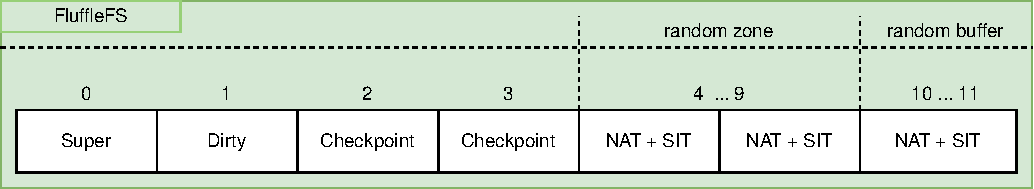
\includegraphics[width=1\textwidth]{resources/images/fluffle-layout.pdf}
	\caption{Fixed and Random zone layouts of FluffleFS.}
    % \includesvg[width=0.6\columnwidth]{resources/images/module-dependencies}
    \label{figure:flufflelayout}
\end{figure}

Consider the fixed zones as depicted in figure \ref{figure:flufflelayout}. In
this region the drive layout distinquishes between three different
datastructures the first two occupying an entire zone.

Firstly, the superblock identifies the filesystem using a magic cookie. In
addition, it remembers the number of zones, sectors and size of sectors the
filesystem should occupy. This metadata allows to identify if the partition was
resized. The superblock is written upon filesystem creation and in principle
never changed. The implication is that the filesystem can not cope with resizing
partitions.

Secondly, the dirtyblock keeps track of filesystem opening and shutdown. The 
block is written upon opening the filesystem and removed once closed completely.
Other datastructures in combination with the dirtyblock allow to identify andmod
checkpoint maintains the wraparound-pointers\footnotemark[13] for both the random
and log zone. Moreover, after the first sector of zone $(n+1) \bmod{2}$ is
written then zone $n \bmod{2}$ is reset. The filesystem can always recover by
reading zone $n$ linearly first and stopping as soon as the first hole is
encountered. In the rare case that zone $n$ sector $0$ is already a hole, the
data must reside at $n+1$ sector $0$. The checkpoint system relies on features
of ZNS that allow to query current write-pointers of individual zones. This
feature allows to identify that sectors are unwritten. To adapt the checkpoints
for use with regular block devices a checksum of the random and log pointers can
be used to prevent against garbage reads.

\footnotetext[13]{FluffleFS manages separate write-pointers from those
maintained by ZNS devices internally as well as wraparound pointers.}

This concludes the data layout as stored in the fixed zone of FluffleFS, the
most straightforward region of FluffleFS. Next, the random zone is used to keep
track of two special management datastructures being NAT and SIT. These have the
same functionality as in F2FS but the datastructures themselves are different.

Firstly, the NAT blocks keep track of inode and \textit{Logical Block Address}
(LBA) pairs. Each LBA can easily be translated to a zone and sector allowing to
determine the location of inodes on the drive. Secondly, the SIT blocks
maintain which sectors of the drive are occupied using bitmaps.

The appending of NAT and SIT blocks in the random zone happens in interleaved
fashion. A special type is stored alongside each block so it can be identified.
When the random zone is filled entirely the data is compacted into the random
buffer. This is done using a iterative method which can be captured in the
following steps.

\begin{enumerate}
    \item Copy from the wraparound-pointer of the random zone the current and
    next zone into the random buffer.
    \item Reset the data from the two zones that have been copied into the
    random buffer.
    \item Update the wraparound-pointer to keep track of the new start of the
    zone.
    \item Write a new checkpoint block to update the random zone
    wraparound-pointer.
    \item Update the write-pointer of the random zone to the newly writeable
    region.
    \item Read the random buffer and transform into set that only keeps
    most recent inode LBA pairs (NAT) and most recent occupied blocks (SIT).
    \item Flush the set to the random zone at the new write-pointer.
    \item Erase the random buffer.
\end{enumerate}

These steps $i$ are repeated for $i = n/2$ times where $n$ is number of zones in
the random zone. FluffleFS assumes that the random zone is of size
$n \bmod 2 = 0$. Clearly, the checkpoints does not store write-pointers only
wraparound-pointers in persistent storage. However, storing those pointers is
unnecessary as they can be recovered by querying the ZNS device. This is
achieved by reading from the start of the wraparound-pointer until the first
hole is encountered. Once again adaptation for regular block devices can be
achieved by adding checksums to the datastructures.

The main limitation of this approach is that it can only compact information
for repeated inodes and occupied blocks per two zones. Should the random zone
contain a linearly increasing sequence data that occupies size $n > 2$ then no
compaction will take place. Such limitations are acceptable as filesystem
recovery and stability features will not contribute towards the research
questions in this work.

This concludes the layout and behavior of the random zone and the accompanying
random buffer. Lastly, we describe the most involved zone of FluffleFS namely
the log zone which also has an accompanying log buffer. An overview of the
layout of these regions is shown in figure \ref{figure:flufflelayoutlog}.

\begin{figure}[h!]
    \centering
	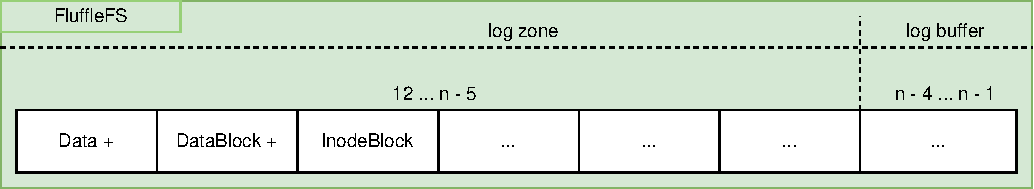
\includegraphics[width=1\textwidth]{resources/images/fluffle-layout-log.pdf}
	\caption{Log zone layout of FluffleFS.}
    % \includesvg[width=0.6\columnwidth]{resources/images/module-dependencies}
    \label{figure:flufflelayoutlog}
\end{figure}

Firstly, the log zone contains three different datastructures that can be
interleaved to an extend. These datatsructures include raw data, data blocks
keeping track of raw data and inode blocks keeping track of inodes and data
blocks. The decoupling of inodes and data blocks reduces write-amplifcation.

For consistency all raw data is always written before the data block that
indicates their existence is. Only after the data blocks are the inode blocks
flushed. Next, the NAT blocks are flushed and finally the SIT blocks. This order
does not prevent data loss during a partial flush but it does prevent
inconsistent states.

Inside a data block is simply a large consecutive list of LBAs increasing
with the order of data. However, the end of a data block contains a LBA which
points to the next data block or zero if it does not exist.

The first data block is found through the inode block by means of an inode
entry. In addition, these entries contain the parent inode, the inode number
itself, the type of inode and the size of the inode entry including the null
terminated name. This null terminated name is placed directly after each
inode entry. Each inode block is a dynamc list of inode entries and names
until no more entries or the name of the newly added inode no longer fits
inside the current block. No optimizations are made to try and balance inode
entries with their names across multiple inode blocks. Finally, inode entries
and names are never stored across inode block boundaries.

The overall layout of an inode block is shown in figure
\ref{figure:fluffleinodeblock}. Importantly, for none of these datastructures
do we have to store type information as the use for each block can be inferred
from the NAT blocks and the subsequent inodeblocks they point to.
A possible improvement includes better capturing this many to one inode to LBA
relation in the NAT blocks instead of storing each inode LBA pair separately.

\begin{figure}[h!]
    \centering
	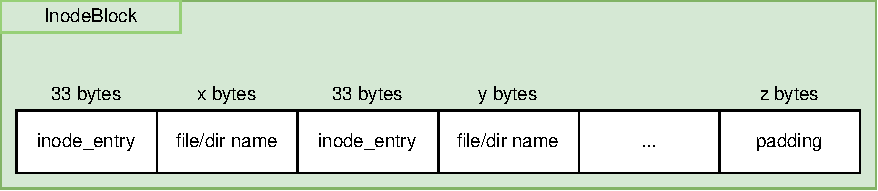
\includegraphics[width=1\textwidth]{resources/images/fluffle-inodeblock.pdf}
	\caption{Layout of an inode block in FluffleFS.}
    % \includesvg[width=0.6\columnwidth]{resources/images/module-dependencies}
    \label{figure:fluffleinodeblock}
\end{figure}

Finally, the log zone also has a log buffer similar to the random zone and
buffer. The same compaction method and limitations apply. This concludes the
layout and behavior as performed for the log zone.

Clearly, all regions combined create a functional data layout that can support
typical filesystem operations such as the creation, deletion of files and
reinitialize after a previous clean unmount.

\subsubsection{Memory}

This next section addresses how the filesystem data is represented in memory.
Firstly, an overview of all these datastructures is given and afterwards their
structure and use. In additon, we describe which in memory representation are
synchronized to the drive and how the translations are performed. Several
techniques are in place to ensure that these in memory representations are
performant as well as easily be synchronized with the drive contents. Primarily,
Red-black self-balancing \textit{binary search tree} (BST)s
\cite{Bayer2004SymmetricBB} are heavily used to ensure datatsructure operations
can be performed with cost $\mathcal{O}(\log n)$.

In total there are eight large datastructures kept in memory by FluffleFS of
which three are used for synchronizing with the drive. In no particular order
these are:

\begin{enumerate}
    \item inode\_nlookup\_map
    \item path\_inode\_map
    \item inode\_lba\_map
    \item open\_inode\_vect
    \item nat\_update\_set
    \item inode\_entries\_map
    \item data\_blocks\_map
    \item snapshots\_map
\end{enumerate}

Most of these datastructures support concurrent access and modification through
the use of wrapper classes. The types of operations and concurrency supported
are detailed in a later section. The datastructures responsible for drive
synchronization include \begin{enumerate*} \item nat\_update\_set 
    \item inode\_entries\_map \item data\_blocks\_map \end{enumerate*}.

FluffleFS predominantly uses maps that map the inode number to specific data,
the algorithm underlying these maps is the mentioned red-black self-balancing
binary search tree. The redundant storing of the same inode number across
maps could potentially be improved at the cost of concurrency for insertions
and deletions.

We briefly explain the contents and use of each datastructure. Firstly, the
\textit{inode\_nlookup\_map} is used to prevent delayed I/O requests from
arriving when an inode has already been renamed or deleted (unlinked). FluffleFS
will only actually remove the stale data from memory once the nlookup count for
that inode reaches zero.

More complex but less important is the \textit{path\_inode\_map}. This
datastructure acts as a cache for recently looked up flushed inodes. In addition
FluffleFS has dedicated datastructures for unflushed data that will be explained
later. \textit{path\_inode\_map} preserves name inode pairs for the children of
a given inode. The structure is demonstrated in figure
\ref{figure:flufflepathmap}. The use of this datastructures allows to perform
lookups in $\mathcal{O}(2 \log n)$ time. It should be noted that normally FUSE
manages its own data and inode caches, however, these are incompatible with
FluffleFS its offloading mechanisms. Due to the high cost and excessive inode
block reading of a lookup
otherwise this cache was implemented. Next \textit{inode\_lba\_map} is shown to
alleviate some of this cost for cache misses.

\begin{figure}[h!]
    \centering
	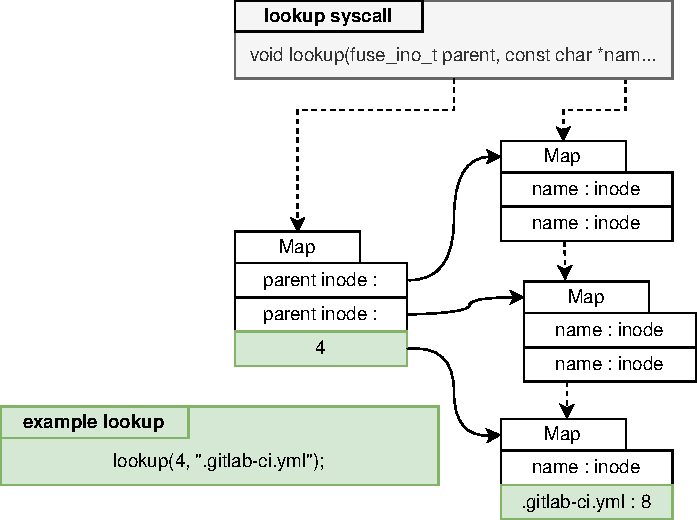
\includegraphics[width=0.7\textwidth]{resources/images/fluffle-path-map.pdf}
	\caption{Structure of path map cache for fast lookups.}
    % \includesvg[width=0.6\columnwidth]{resources/images/module-dependencies}
    \label{figure:flufflepathmap}
\end{figure}

This \textit{inode\_lba\_map} maps inode numbers to a small datastructure that
retains the inode number, its parent inode number and a mutex. The main purpose
of this datatsructure is to quickly evaluate if an inode exists on the
filesystem. In addition, the parent inode number reduces the cost of
\textit{path\_inode\_map} misses since we can find all children of an inode at
cost $\mathcal{O}(n \log n)$. This is substantially lower than having to find
the LBA of each inode and reading the entry from the drive at cost
$\mathcal{O}(n + (n \log n))$ especially as \textit{inode\_lba\_map} prevents
reading from the drive entirely.

Once the inode is located and its existence is verified the next steps of
operations can begin. For typical operations such as reading and writting
FluffleFS must keep track of files opened. This is done through
\textit{open\_inode\_vect}. For every opened file a unique file handle is
created that is associated with the inode, calling PID and the flags from the
\textit{open} call. For every subsequent call this unique file handle will allow
FluffleFS to find the relevant information. This datastructure is necessary
because in \textit{release} and \textit{close} calls it will otherwise not be
possible to determine the calling PID.

This concludes the datastructures that provide runtime operations and are solely
represented in memory. The next three datastructures are used to synchronize
with the drive contents and the final datastructure is solely for offloading.

Firstly is \textit{inode\_entries\_map} this datastructure keeps unflushed
\textit{inode\_entries} and name pairs in memory. The absence of this entry on
the drive is reflected by a zero lba in the \textit{inode\_lba\_map}. Potential
triggers for flushing this datastructure include calling fsync, entries reaching
the size of one inode block or based on a timer. An overview of these different
access patterns for in memory and flushed inode data is shown in figure
\ref{figure:fluffleinodesync}. The result of the linked map structure is that
lookups for unflushed data will be substantially faster than flushed
with $\mathcal{O}(2 \log n)$ compared to $\mathcal{O}(n)$ respectively.

\begin{figure}[h!]
    \centering
	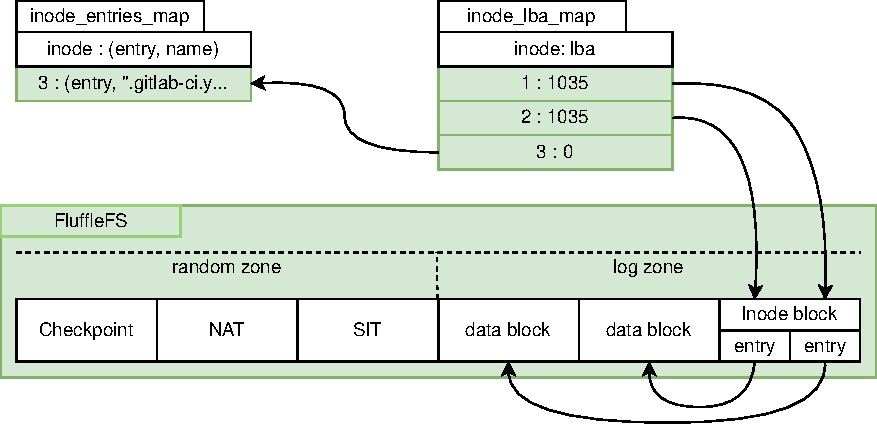
\includegraphics[width=0.7\textwidth]{resources/images/fluffle-inode-sync.pdf}
	\caption{Inode entries synchronization.}
    % \includesvg[width=0.6\columnwidth]{resources/images/module-dependencies}
    \label{figure:fluffleinodesync}
\end{figure}

For unflushed inodes this \textit{inode\_entries\_map} works together with the
\textit{data\_block\_map} that keeps track of unflushed data blocks. Such data
blocks are linked together and numbered in the corresponding map. Finding the
data block number and index inside the block are governed by the following
formulas where $S$ is the size of a sector in bytes, the block number and index
are represented $d$, $i$ respectively and $o$ is the I/O offset in bytes.

$$d = (o / S) / (S - 8) /8$$
$$i = (o / S) \bmod{(S - 8) /8}$$

For accessing subsequent data blocks on the drive all previous blocked must be
accessed to obtain the next block with corresponding complexity
$\mathcal{O}(n)$. While in memory the \textit{data\_block\_map} allows for
accesses of $\mathcal{O}(2 \log n)$. Still this design of linked data blocks is
strongly unrecommended and has a severe flaw causing significant write
amplifcation. Should the last data block of a particular inode be rewritten due
to file changes then every other data block needs to be rewritten as well.
Consider a write to the tail of a file size 1GiB on a drive with 4KiB sectors
then this will result in 512 data blocks being rewritten. This flaw is
circumvented by creating a datastructure similar to NAT but for data blocks
instead of inodes. This feature is not implemented as it does not contribute
towards the research goals in this work as well as being impeded by time
constraints.

A comparison of both in memory and on drive representations of data blocks
is shown in figure \ref{figure:fluffledatablock}.

\begin{figure}[h!]
    \centering
	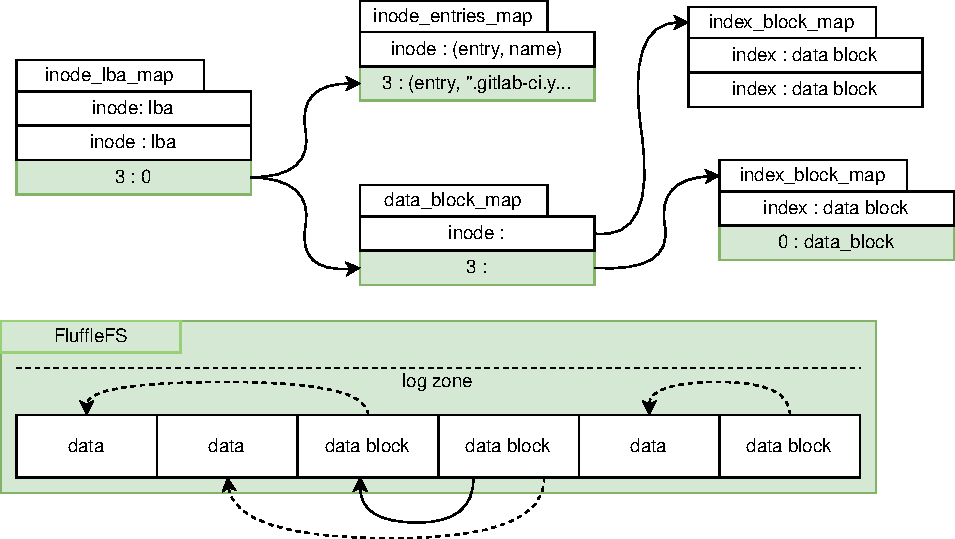
\includegraphics[width=0.7\textwidth]{resources/images/fluffle-data-block.pdf}
	\caption{Data block layout in memory and on drive.}
    % \includesvg[width=0.6\columnwidth]{resources/images/module-dependencies}
    \label{figure:fluffledatablock}
\end{figure}

Lastly are \textit{nat\_update\_set} and \textit{snapshots\_map} these will be
explained in subsequent sections. This concludes the synchronization
datastructures and the datastructures altogether. Overall the datastructures
form a layered but cohesive representation of the state of the filesystem. The
next section we show how different operations access and modify data step by
step.

\subsubsection{Operational Rules}

In a filesystem substantial effort goes into designing the individual steps of
each operation and all their possible concurrent interleavings such that
together they still guarantee properties such as consistency and atomicity.
Similar effort and design steps have been taken for FluffleFS in which we
identify five individual operations. Moreover, in the subsequent section these
steps are extended such that the support concurrent operation. Firstly, the
five primary operations of FluffleFS include:

\begin{enumerate}
    \item Looking up a name within a directory, \textit{lookup}
    \item Creating a new inode, \textit{create}
    \item Resizing a file, \textit{ftruncate}
    \item Reading a file, \textit{read}
    \item Writting a file, \textit{write}
    \item Synchronizing filesystem with drive, \textit{fsync}
\end{enumerate}

Among these are several sub-operations that are repeatedly performed by the
previous operations. These include \begin{enumerate*} \item Verifying an inode
exists \item Verifying data blocks exist \end{enumerate*}. Firstly, the
inode verification works by:

\begin{enumerate}
    \item Checking the inode is non zero as this is reserved while 1 returns
    hardcoded data about the filesystem root directory. 
    \item Looking up the inode in \textit{inode\_lba\_map}. Upon failure the
    inode does not exist.
    \item Lookup the inode in \textit{inode\_entries\_map}, it might be that a
    recent update has changed information about the inode but it has not been
    flushed to the drive. If the entry exists its data is returned immediately.
    \item If the inode was not in \textit{inode\_entries\_map} than by induction
    the inode lba in the \textit{inode\_lba\_map} will be non-zero and the inode
    block is retrieved from the drive.
    \item The inode entry is found in the retrieved inode block along with its
    name, should it not, a critical error will be raised as the filesystem has
    then become inconsistent.
\end{enumerate}

To reduce the cost of the verify inode function it also retrieves the most up
to information about the inode. This includes its type, name, size and parent.
A special \textit{inode\_stat} support function converts the result from this
inode information to a format native to FUSE.

Next the verifcation of a data block is similar but slightly less involved:

\begin{enumerate}
    \item First \textit{data\_blocks\_map} is accessed to see if there are
    unflushed blocks for the given inode.
    \item If so the map is traversed to see if it contains the specific block
    number as only recently updated unflushed blocks are in the map. If it is
    there the data block is returned from the \textit{data\_blocks\_map}
    directly.
    \item Otherwise the data blocks on the drive are traversed until the
    block for the request block number is found. Any failure to access any block
    will result in an immediate critical error as it indicates the filesystem
    is inconsistent. It is the callers responsibility to verify the file is
    sufficiently sized such that the specified data block numbers should
    actually exist.
\end{enumerate}

In addition to verifying the existence of the data block this procedure, similar
to the inode verification procedure, also returns the appropriate data along
side it. From now on forward these two procedures for inode and data block
verification will be referred to as \textit{get\_inode} and
\textit{get\_data\_block} resepectively. In addition, \textit{inode\_stat}
implies the calling of \textit{get\_inode}.

We now turn to the first of seven main procedures of Flufflefs, \textit{lookup}:
\begin{enumerate}
    \item First \textit{inode\_stat} is performed on the parent inode supplied
    as argument to \textit{lookup}. In addition \textit{lookup} specifies a name
    argument as well. Should this fail an \textit{ENOENT}\footnotemark[14] error
    will be returned.
    \item Next \textit{path\_inode\_map} is traversed to see if the inode name
    for the particular parent exists.
    \item Should it not the \textit{inode\_lba\_map} is iterated to find to
    all inodes with the specified parent.
    \item For each of these inodes the inode entry is read from its inode block
    on the drive to see if those inodes bare the specified name.
    \item If the name could not be found using either method \textit{ENOENT}
    is returned.
    \item Should it exist then \textit{inode\_stat} is called on the name
    matching inode and this data is returned.
\end{enumerate}

\footnotetext[14]{UNIX error codes are used to indicate the types of failure
in FUSE as they are return statusses to system calls, A complete overview can
be found through man either online \cite{errno} or by executing 
\textit{man errno}.}

The calling of \textit{lookup} is managed by FUSE automatically when directories
are traversed or before files are \textit{opened}. This \textit{open} procedure
is not described in detail as it is effectively \textit{inode\_stat} in
combination with creating an entry in \textit{open\_inode\_vect}.

Next is the creation of inodes:

\begin{enumerate}
    \item First the name is checked to be below the maximum permissable length.
    This is dominated by the sector size as the inode entry and name pair must
    fit unto a single inode block. If the name is to long the error
    \textit{ENAMETOOLONG} is returned.
    \item Next the existence of the parent inode is verified using 
    \textit{inode\_stat} as well as ensuring that it is a directory.
    If not \textit{ENOENT} or \textit{ENOTDIR} is returned respectively.
    \item Each directory can only contain one inode of a particular name, this
    is checked by performing \textit{looukp}. If it already exists
    \textit{EEXIST} is returned.
    \item Now the inode creation starts by incrementing the \textit{inode\_ptr}
    and assigning the previous value to the new inode.
    \item The relevant information such as type and parent are inserted into
    \textit{inode\_entries\_map}.
    \item Next the new inode information is added to \textit{inode\_lba\_map}
    and finally to \textit{path\_inode\_map}.
    \item Finally, in the case of a file a file handle is created and 
    added to \textit{open\_inode\_vect} as \textit{create} should immediately
    \textit{open} a file.
\end{enumerate}

Once a file is created it can potentially be resized using the
\textit{ftruncate} procedure:

\begin{enumerate}
    \item The existence of the inode is verified using \textit{get\_inode} if
    it does not exist \textit{ENOENT} is returned.
    \item Next the inode is verified to be a file and otherwise \textit{EISDIR}
    is returned.
    \item The next steps are based on if the size of the file is increasing or
    decreasing.
    \item For decreasing, the data blocks are removed to match the size and the
    sectors previously occupied by this data and metadata are marked reclaimed.
    \item For increasing, the non-existing data blocks are created.
    \item Finally, the size of the inode is updated and the changes are added
    to textit{inode\_entries\_map}.
\end{enumerate}

The next two operations are arguably the most important procedures of any
filsystem being \textit{read} and \textit{write} operations. Firstly,
\textit{read} works by:

\begin{enumerate}
    \item Verifying the inode exists with \textit{get\_inode} and checking the
    offset is not beyond the file size.
    \item Next the size argument is adjusted to prevent reading beyond the file
    size. If the remaining size is zero the procedure returns immediately with
    zero bytes of data.
    \item Next the initial data block number and data block index are determined
    from the read offset. This block is fetched using \textit{get\_data\_block}
    \item Each of the sectors specified by the data block is read into a buffer
    if at any point the data block index reaches its maximum the next data
    block is fetched. Any request with an error be it for data or data
    blocks will make the procedure return \textit{EIO}.
    \item If all data was read into a buffer succesfully this buffer is
    returned. The data returned from this buffer is adjusted by the offset
    modulo the sector size to adjust for unalignment.
\end{enumerate}

The \textit{write} operation is fairly similar but has slightly different
nuances and conditions. The final operation is \textit{fsync} and while its
operation has been implemented it is not actually used in the current state
of FluffleFS. The \textit{fsync} operation essentialy consists of flushing
or synchronizing datastructures to the drive in an order that has good
consistency guarantees.

\begin{enumerate}
    \item First, all data blocks that \textit{are new or have pending changes}
          (unsynced) are flushed to the drive. These contain metadata about
          which blocks are stored at what LBA.
    \item Next, all unsynced inodes flushed to the drive. Each inode contains the
          LBA of its first data block.
    \item Lastly, all NAT and SIT blocks are updated to reflect these changes.
\end{enumerate}

Should the drive be out of free space during any of these operations either the
garbage collection for the log zone or the rewritting of the random zone will
be performed and the operation will be repeated.

All these operations together form the majority of the FluffleFS filesystem.
This shows a practical implementaton of our design that adheres to the
requirements set out for concurrent regular and offloaded filesystem access on
CSxs. The degree of concurrency and how this is achieved is described in the
next section.

% These procedures can be classified between \textit{externally} and
% \textit{internally} facing. Here externally facing create the appropriate
% response that FUSE expects for each request. Contrarily, internally facing
% procedres simply return what error they deem should be returned if any but don't
% call the FUSE runtime directly. This layered system is needed as a FUSE response
% can only be returned once per system call. The result is that an externally
% facing procedure can call any internally facing procedures but never another
% extern one. The differentation between these types of procedures allows to
% significantly reduce duplicate code where that would otherwise not have been
% possible.

% No unlink and rename functionality, unmarking / reclaiming of blocks not
% performed.

\subsection{Concurrency}

The use of snapshots allows for concurrent regular and offloaded access to the
same file. This is achieved by ensuring the data pointed to in the snapshot
is immutable during the execution of kernels. We guarantee this immutability by
not using in-place updates. Instead all write go to the tail of a log. Until now
no other work has been able to provide this much concurrency for CSxs with
filesystem integration. However the entire framework still needs to use several
locking mechanisms across various parts to ensure correct operation.

\subsubsection{Fine-grained Locking}

These include a global multi-reader single-writer (MRSW) lock for filesystem
operations, a mutex per inode, a mutex for SPDK requests, a mutex for the uBPF
vm and a MRSW lock for each of the FluffleFS datastructures.

The use of MRSW locks allows some operations to happen concurrently (multi read)
while allowing sequential operations for another (single write). By using this
type of lock for filesystem operations it is possible to allow most to happen
concurrently. Only intricate filesystem operations such as flushing or garbage
collection have to be performed sequentially.

Due to the concurrency for most filesystem operations indivudual datastructures
also have their own MRSW locks. These prevent typical problems with non
thread-safe when performing operations such as insertion or deletion in
parallel. Furthermore, by using a MRSW lock read operations on these
datastructures can still happen concurrently potentially improving performance.

Far simpler are the mutexes for uBPF and SPDK as these simply block any call
until the previous one has completed. This simple approach has several
limitations that can be resolved in future work. These limitations are addressed
in the \textit{considerations} section.

Lastly, there is a mutex per inode that gets locked just before the current
information about the inode is retrieved. However, these locks are only used for
regular access. This can be done without risk as the snapshot is made when the
extended attribute gets set and these snapshots already store all required
information about the inode.

Clearly OpenCSD \& FluffleFS are able to have many of their operations be executed
concurrently using fine-grained locking. Implementing concurrency is important
given the prevalance of many-core systems and the asynchronous nature of I/O
operations. We argue that is unlikely to achieve comparable performance to other
flash optimized filesystems without it.

\subsubsection{Performance Instrumentation}

Such a performance comparison requires measurement and instrumentation. Here
there is often a steep trade-off between the performance impact and the amount
telemtry that can be recorded. OpenCSD uses a boundless lockless
queue \cite{Michael1996SimpleFA} that has low overhead for concurrent insertion
thereby optimizing to reduce the instrumentation impact.

The instrumentation in the OpenCSD framework provides the median, minimum and
maximum execution time of individual functions. While not used during the
performance evaluation itself this instrumentation provides valueable insights
especially during development.

\subsection{Offloading}

By far the most important part of a CSx is the system to offload execution on
the device. However, the degree of user programmability strongly various in
computational storage \cite{lukken2021past}. It is in this offloading that we
find the most predominant contribution of our work.

As set out in our design this offloading process requires three fundamental
features. Firstly, the use of extended attributes alongside the calling process
its PID. Secondly, the use of an universal ISA with call support to trap
into vendor code. Lastly, safety such as memory access validation and static
verification should be possible. The next section describes how each of these
features is implemented. Afterwards, the entire offloading process is described
as a whole.

\subsubsection{Extended Attributes}

Firstly is registering which file operations should be offloaded through
extended attributes. As per design these associations are managed on a per
process level. Trivially one would simply get the PID for each incoming I/O
operation and determine the appropriate action. However, this is not
possible due to the absense of the PID from the call information for special
operations such as \textit{release} and \textit{close} in FUSE. 

Instead our implemenation maintains two datastructures one 
\textit{open\_inode\_vect}, explained previously, and a \textit{snapshots\_map}.
Here the entries in the \textit{snapshots\_map} can be correlated to the open
files in \textit{open\_inode\_vect} through PID inode pairs. In addition the
\textit{open\_inode\_vect} contains a unique \textit{file handle} (fh) that is
monotonically incremented for each call to \textit{open}. It is through this
\textit{fh} that any current snashots for the process calling \textit{close}
can be correctly cleaned up. This overall process is shown graphically in
figure \ref{figure:offloadingmanagement}.

\begin{figure}
    \centering
	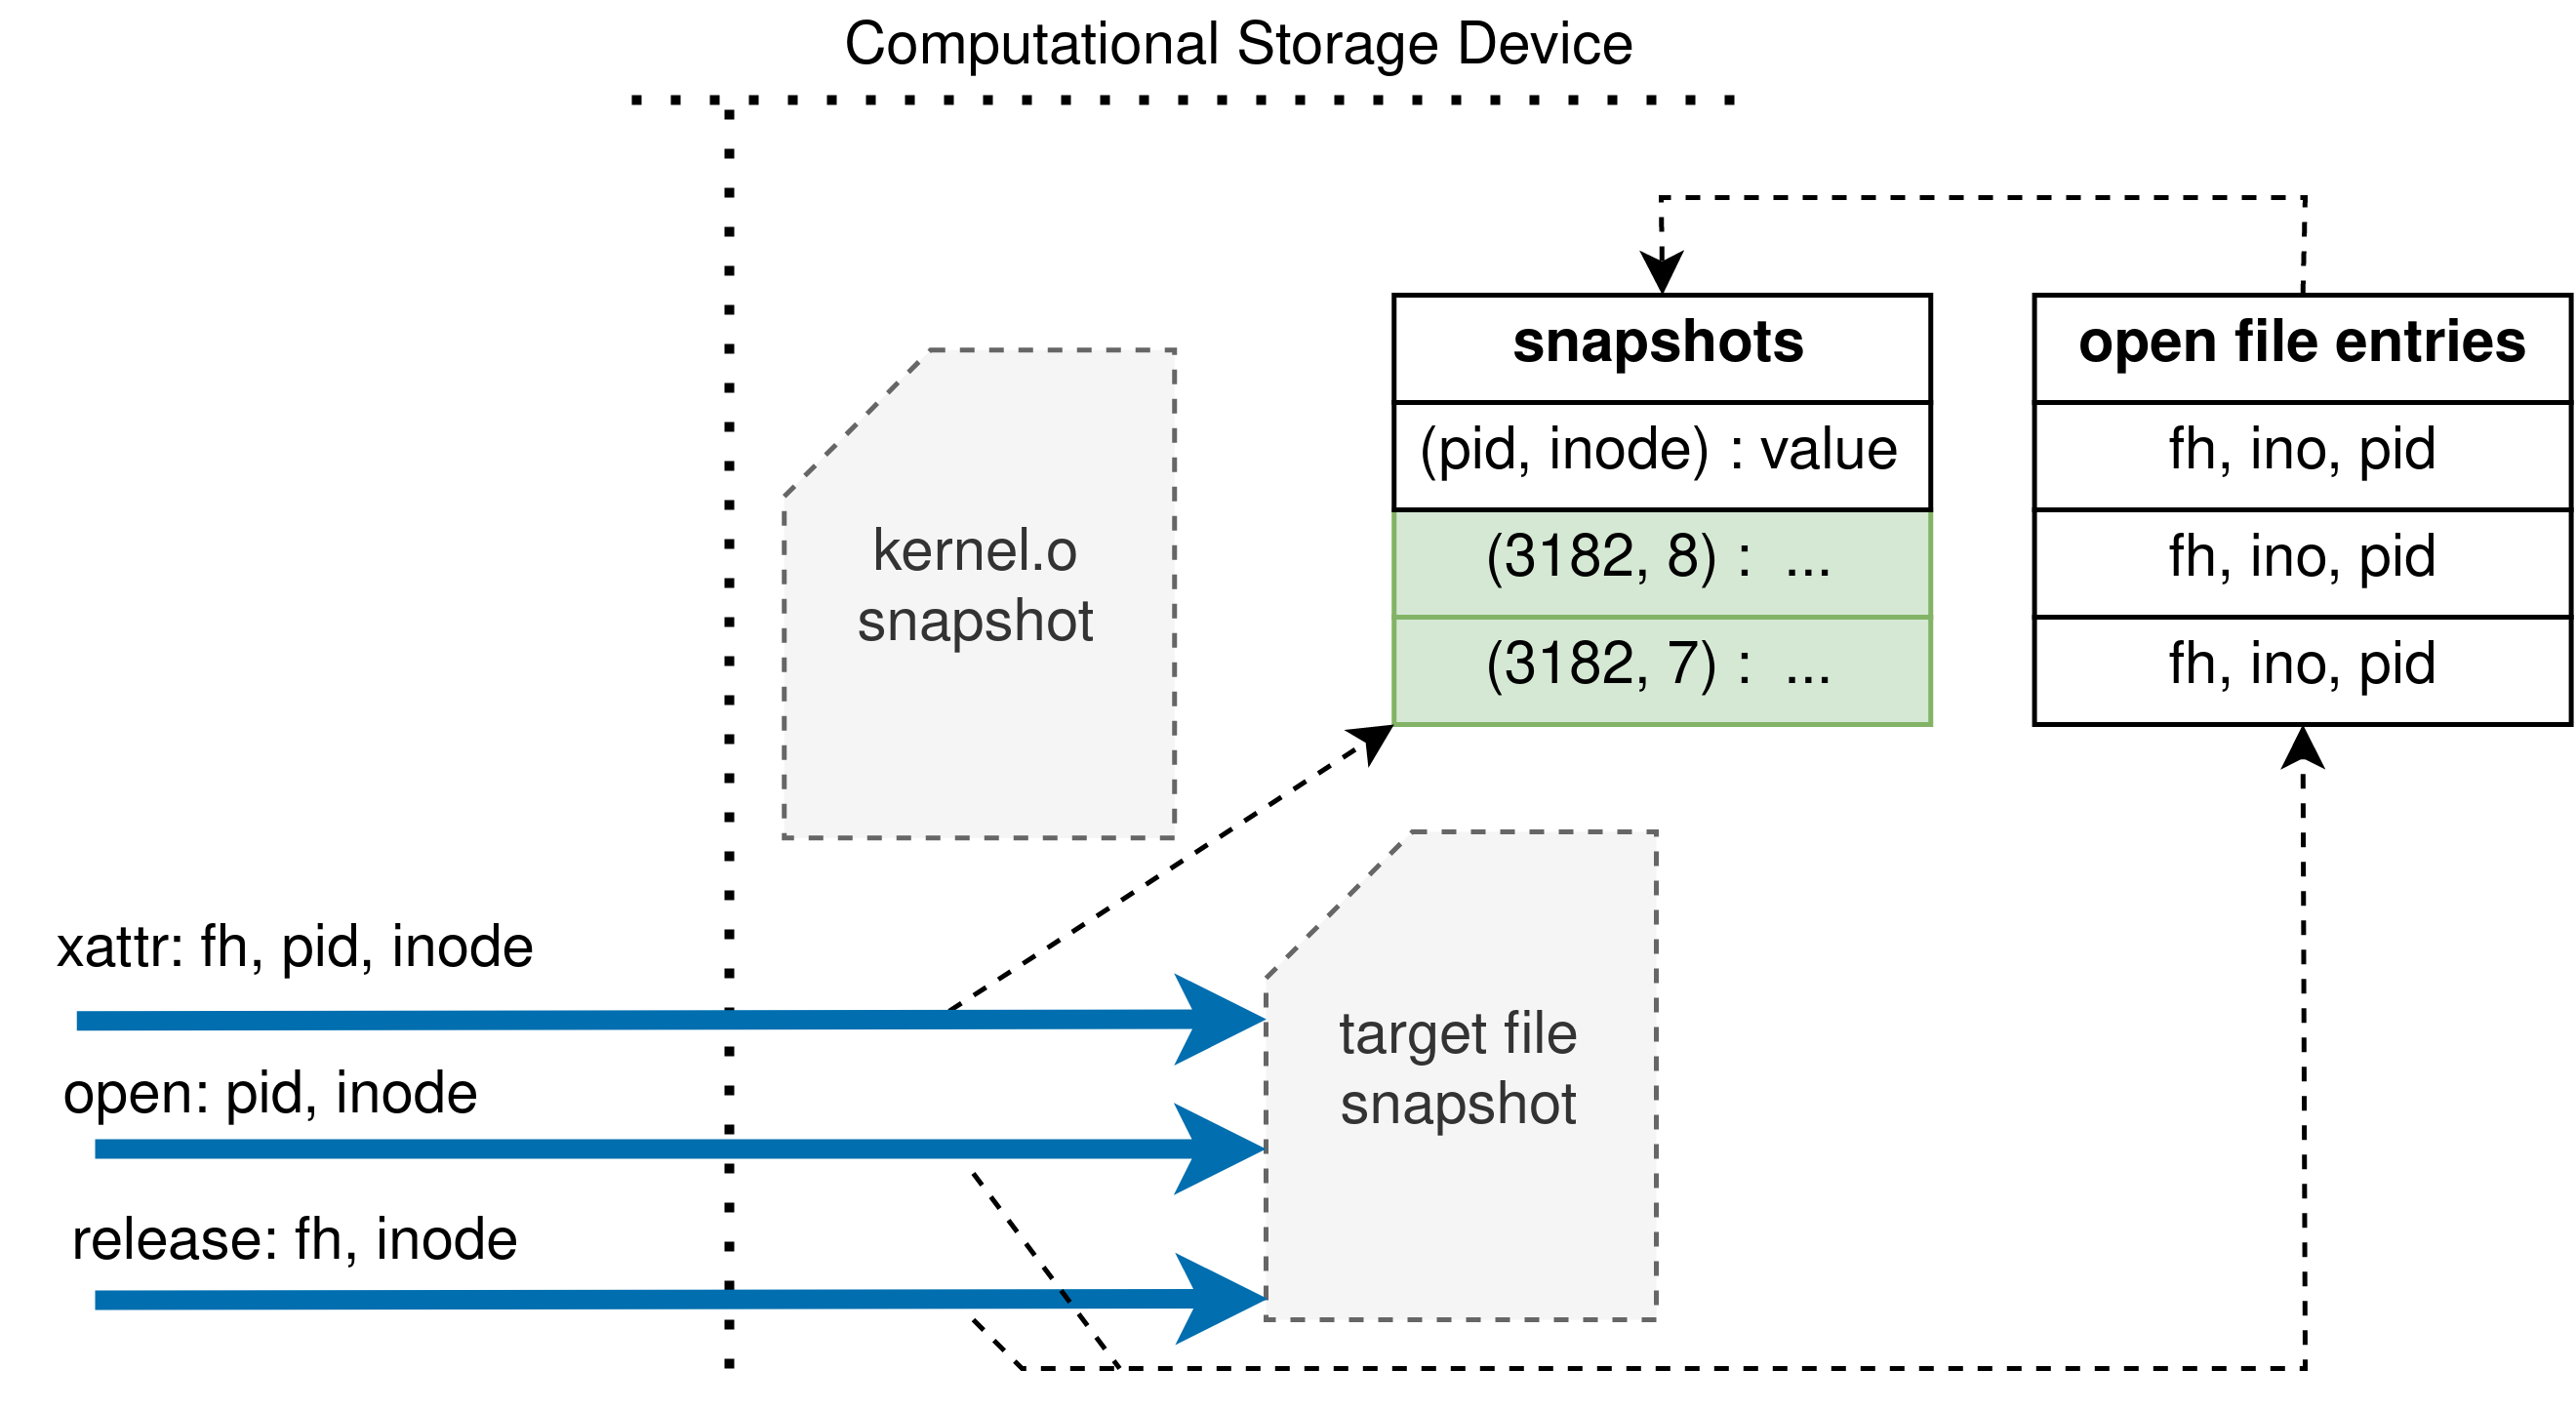
\includegraphics[width=1\textwidth]{resources/images/offloading-management.png}
	\caption{Identifying registered kernels across various system calls}
    % \includesvg[width=0.6\columnwidth]{resources/images/module-dependencies}
    \label{figure:offloadingmanagement}
\end{figure}

Beyond this PID inode pair the \textit{snapshots\_map} maintains four snapshots
for each possible type of offloading operation and the snapshot for the target
file. In turn each of these snapshots is just the inode and data block
information reusing the already existing datastructures to represent these.
The four types of offloading are \begin{enumerate*} \item read stream
\item write stream \item read event \item write event \end{enumerate*}.

For each of these types of offloading a key is chosen that identifies which
offloading procedure to perform. These are
\textit{user.process.csd\_read\_stream},
\textit{user.process.csd\_write\_stream} \textit{user.process.csd\_read\_event}
and \textit{user.process.csd\_write\_event} resepectively. Of these
\textit{user.process.csd\_read\_stream} and
\textit{user.process.csd\_write\_event} have arguably the most practical 
applications.

\subsubsection{Types of Offloading}

The behavior of these offloading types is different between read and write as
well as stream and event. Read offloads are given an empty buffer to store and
return data to the host through. Contrarily, Write offloads are given a buffer
that contains the user provided data. The size of these buffers depends on the
type of offloading as with stream offloads it matches the size of the I/O
request. For instance, if a \textit{read} system call is performed at offset
512000 with size 4096 then the buffer will be 4096 bytes in size as well.

For \textit{event} offloads user or system configuration might be required to
determine apppropriate buffer sizes. We will first explain the behavior of event
and stream offloads.

with \textit{stream} offloads the I/O operation is performed by the user
submitted kernel with data such as the location of data blocks, the size and
offset of the request. How much of the data from this I/O is returned to the
host or actually written is determined by the user submitted kernel. For write
requests the return data of the kernel can be used to determine the final size
of the file if it deviates from the I/O request. For \textit{stream} the most
trivial kernels are \textit{passthrough} that have exactly the same behavior as
if the filesystem where performing the request.

\textit{Event} offloads are more complicated. These first let the regular I/O
request complete and run on the data that was read or written. The result is
that they return or write additional data. For writes this can introduce
substantial complexity that can largely be mitigated by only allowing appending
writes to the end of the file. The most trivial implementation of this will
simply refuse to launch the event kernel if the reguarl I/O request is not
performed up until or beyond \textit{End Of File}(EOF). Given that the regular
I/O request must first complete \textit{event} offloads suffer from additional
data movement and latency while waiting for this request roundtrip over busses
such as PCIe. We will address this issue with a potential solution in our
consideration section.

While the difference between these types of offloading is subtle both have
substantially different practical applications. In addition, certain behavior
would be hard to implement effectively without these different types. Clearly,
the different types of offloading create a flexible user-programmable system
overall.

\subsubsection{uBPF}

As mentioned previously uBPF \cite{ubpf} is used to perform the execution of
user-programmable aspects of our system. This section describes additional
detail about how uBPF works as well as what types of operations we have
implemented through uBPF. Finally, the setup and teardown of the uBPF VM is
described in the next operation section.

Firstly, some additional details about uBPF with some brief reminders. By using
uBPF we are able to define specific operation behavior and have the user
submitted programs trap into these operations optionally with arguments. The
underlying ISA, eBPF, has this capability by supporting special
\textit{syscall} instructions. This call instruction can be hooked to an
operation defined outside of the uBPF VM. The types of operations supported in
our uBPF environemnt are defined firstly by a generic header (\textit{OpenCSD})
and secondly by a filesystem specfic header (\textit{FluffleFS}). Again, tying
operations defined in headers to trapped instructions without exposing the
underlying binary code or firmware is known as an
\textit{Application Binary Interface} (ABI). Like previously, as graphical
representation of uBPF is shown in figure \ref{figure:ubpf-abi2}.

\begin{figure}
    \centering
	\includegraphics[width=0.8\textwidth]{resources/images/ubpf-abi.pdf}
	\caption{Achieving vendor agnostic \textit{Application Binary Interfaces}
        (ABI) through uBPF.}
    % \includesvg[width=0.6\columnwidth]{resources/images/module-dependencies}
    \label{figure:ubpf-abi2}
\end{figure}

Because of this decoupling, practical implementations of a CSx will have uBPF VM
reside in vendor firmware on the device. This firmware would also contain the
instructions for each of the operations defined in the generic and filesystem
specific header. Vendors will not have to provide any binary or firmware for end
users to use this system. However, a firmware updating mechanism might be
required for long time support. This decoupling allows for vendor agnostic
kernels without complications around intellectual property. However, such
filesystem specific operations are cumbersome for vendors to implement given the
large amount of modern filesystems. We will address this issue in the
consideration section by proposing a mechanism for
\textit{filesystem agnostic kernels}.

Across our two headers, the generic header contains zero datastructures and
eight operations. Of these operations three are related to performing tasks
while five are related to retrieving information about the state of the VM and
drive.

Furthermore, the filesystem header is more complicated with two enums, five
datastructures and three operations. Across uBPF, the CSx and the host the
endianness of such datastructures needs to be explicitly taken care off. Lastly,
the operations for this filesystem header are for LBA conversion and extracting
data block information. Due to the use of a X86 host architecture and eBPF no
explicit datastructure conversion is implemented in OpenCSD as these both have
the same endianness.

Together these operations and datastructures allow to exchange necessary data
between the host and CSx as well as offload tasks that the host would
otherwise perform. While minimal we show in the result section that this set of
operations is capable of performing practical applications all be it in a
simulated setting.

\subsubsection{Operation}

With implementation details described we can finally show how the entire
offloading operation is performed. This section not only describes what steps
end users need to take to perform an offloaded I/O operation but also what
internal behavior is triggered for each step within OpenCSD and FluffleFS.

The process is shown using distinct steps taken by an end-user. However, the
compilation of source code into eBPF bytecode (kernel) is omitted. This process
is shown in figure \ref{figure:offloading} here each of the bold blue numbered
arrows indicates a distinct ste by the user.

Given that our prototype achieves offloading entirely reusing existing APIs each
step is a system call that traps into the kernel.

Firstly, the \textit{stat} call allows to retrieve information about a file or
directory. Most important, this information contains the inode number as managed
by the filesystem. Such an inode number is a unique identifier within a given
filesystem. As shown this \textit{stat} call is executed on the compiled eBPF
bytecode stored in a file on the FluffleFS filesystem, this file is called
kernel.o in our figure. This \textit{stat} call is essentialy stateless and does
not create any notable internal behavior within OpenCSD and FluffleFS.

Next, the user opens the file for reading or writting using the \textit{open}
call. The file on which this \textit{open} is performed is the file that will be
offloaded called \textit{target file} in this example. When \textit{open} is
called FluffleFS will create an internally managed file handle that uniquely
associates the file handle to the PID of the calling process. It should be noted
that these file handle numbers while monotonically increasing are entirely
distinct from file descriptors as used by unix processes. Furthermore, they are
purely for filesystem inernal state management.

Third, the \textit{setxattr} call is used to set the extended attribute on the
target file with as key "user.process.csd\_read\_stream" and as value the inode
number from the kernel.o file. As soon as this is called FluffleFS creates a
snapshot of the kernel.o file and the target file. In addition, the target file
snapshot is stored in a specific slot for read stream operations. This allows
the snapshots for other operations to occur at different moments in time with
potentially different file contents.

Lastly, is the actual \textit{read} or \textit{write} call. Nix based operating
systems contain many calls to perform this behaviour but our example focusses
on the ones using an offset and size. Upon this call FluffleFS will detect that
the particular inode and PID pair are configured for offloading. It will access
the relevant metadata from the snapshots datastructure and retrieve the
location of data blocks corresponding to the size and offset of the request.
This data is passed to the \textit{NVME\_CSD} module of OpenCSD as it is
responsible for managing offloading state with uBPF. This module creates a new
instance of uBPF as well as some memory space after obtaining a lock. Next the
state and metadata extracted from snapshots is placed at the beginning of this
reserved memory sppace. After which the bytecode of the kernel is read utilizing
the metadata from the snapshot. Finally, the uBPF VM can be started using this
bytecode at which point it starts executing. Upon the creation of the uBPF VM
each of the operations defined in the header are hooked up to implementations.
Since each specific operation is associated to a specific call number this
system is similar to key value pairs. Everytime the user provided eBPF kernel
executes such an operation the execution is trapped and the implementation of
the operation starts executing. Upon return execution is returned to the kernel.
The execution of the kernel is fully terminated once it returns from main. To
return data from the kernel back to the host a special operation is used. The
implementation of this operation essentially performs a copy of a memory segment
from the reserved memory space into a host controlled area. This mechanisms of
copying and moving data will be different in the case of practical
implemenations where data has to be moved over busses such as PCIe. Once the
kernel has finished and the data has been moved the uBPF VM is cleaned up. Due
to the use of anonymous callbacks only one instance of a uBPF VM can be active
within a single process at a time. This is why a lock is used within
\textit{NVME\_CSD}.

\begin{figure}
    \centering
	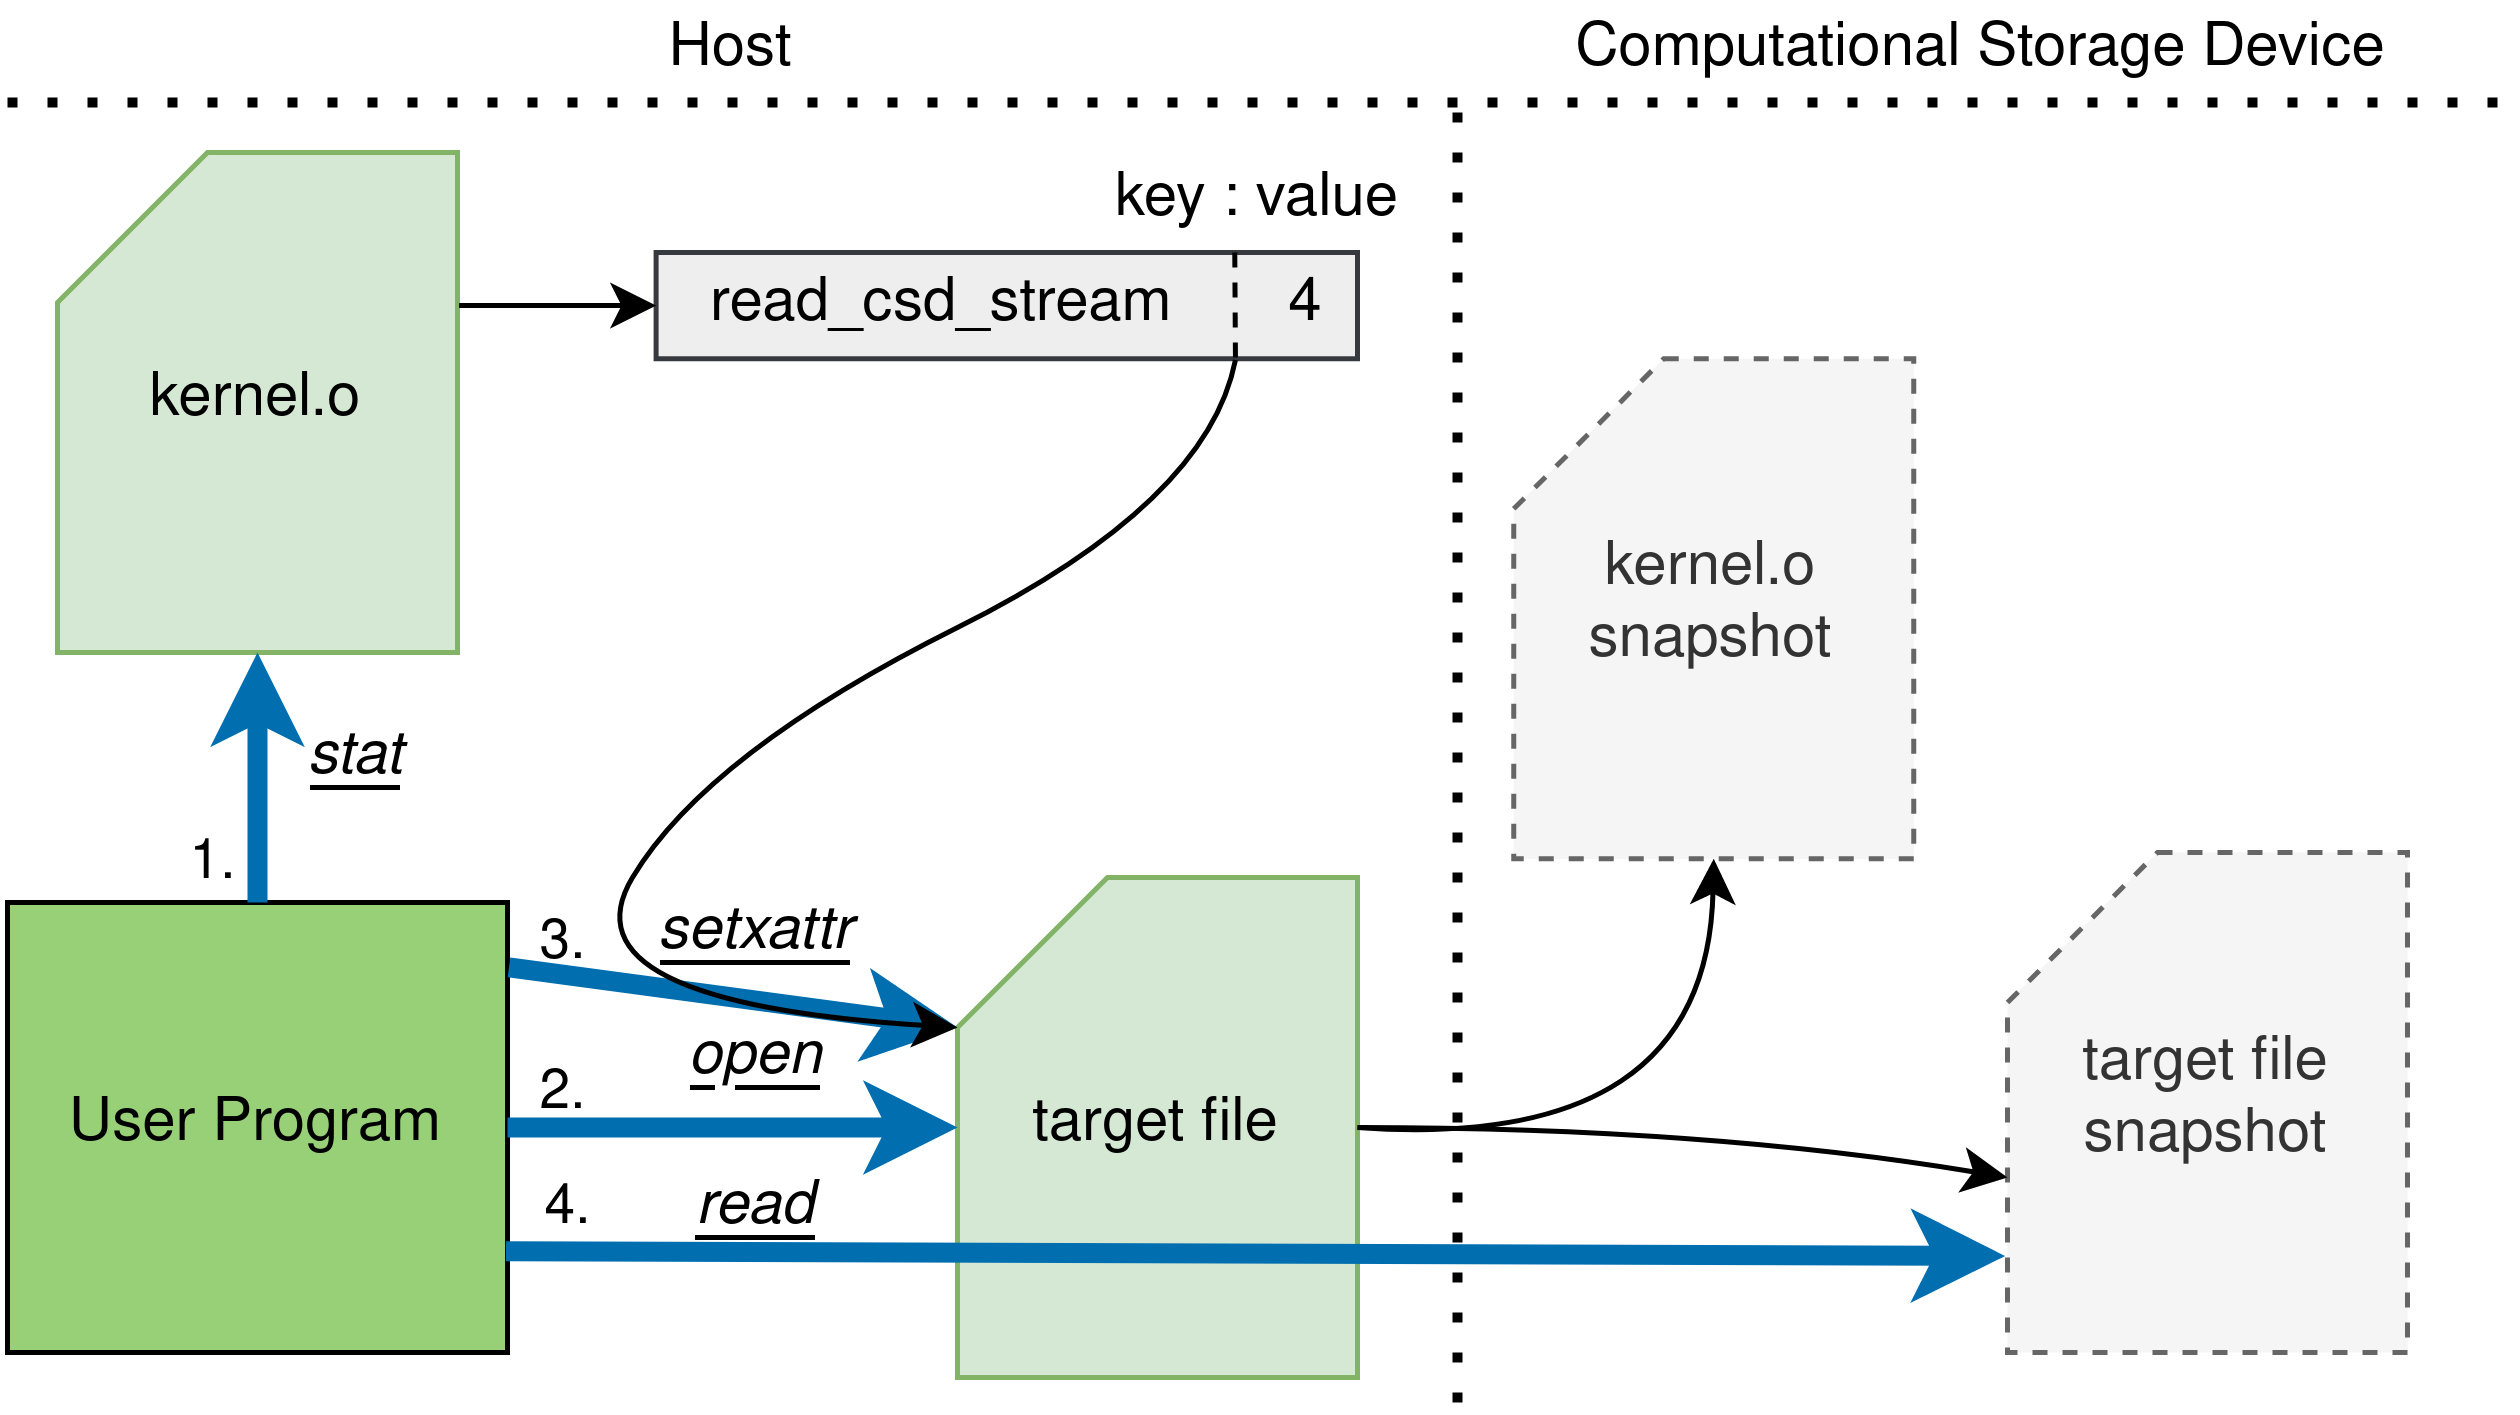
\includegraphics[width=1\textwidth]{resources/images/offloading.png}
	\caption{Core offloading mechanism through extended attributes (xattr)}
    % \includesvg[width=0.6\columnwidth]{resources/images/module-dependencies}
    \label{figure:offloading}
\end{figure}

\section{Iterations}

This section is covered separetely to prevent clutter in the overall design and
implementation sections. Here the distinct iterative changes made throughout the
research project are described on an individual basis. Our process consisted of
four destinct iterations. Two relating primarily to the framework, one to the
filesystem and one to offloading. This section describes each iteration briefly
before going in more detail. Firstly regarding framework iterations we see the
distinct decision to switch from a multi process architecture using mmap for
shared memory maps to a monolithic application. The second iteration lead to
switching away from the design of an accelerator API, much like Vulkan
\cite{vulkan} or OpenCL, to an artificial extension to the NVMe namespace.
The third iteration changed the use of rtld\_next \cite{rtldnext} to creating
an actual filesystem with FUSE. Lastly, as computational storage API our work
switched from using \textit{Portable Operating System Interface} (POSIX)
fadvise \cite{fadvise} to extended attributes (xattr).

For each of these four iterations the advantages of the change as well as the
major issues with the previous solution are described. Each iteration is
described in the same order as previously defined.

\subsection{Shared Memory Monolith}

Modern operating systems offer fastly different methods to write sofware. From
kernel modules, to distributed processes, UNIX pipes and shared memory maps.
Choosing the right model impacts practicalities such as the amount of
development effort required and the robustness of the final solution. 
Furtermore, depending on the software architecture some solutions will be better
suited than others.

During the design the use of shared memory maps was replaced with using regular
shared memory. While both solutions provide shared memory they are fundamentally
different. A shared memory map is a file, leveraging the well known UNIX
principle \textit{everything is a file}, that allows two or more processes to
share a region of memory. While regular shared memory is limited to a single
process, however, this memory could be shared across additional threads.

this single process shared memory solution is one of the most common found in
software today. The concepts of such a program are very well understood as
well as the development using imperative languages being straightforward.

While shared memory maps are typically found in device drivers, such as those
for graphics cards, their use consistutes severe additional development effort.
In conjuction with our design being a simulation there is no scientific value in
using shared memory maps for our design. However, for production ready
implementations this decision needs to be reevaluated.

\subsection{NVMe Namespace Command Set}



\subsection{FUSE Filesystem}

% LD\_PRELOAD / RLTD\_NEXT

\subsection{Extended Attributes}

% POSIX fadvise, does not reach filesystem

% ---------------------------------------------------------------------------
% ----------------------- end of thesis sub-document ------------------------
% ---------------------------------------------------------------------------